\chapter{Methods}

The method of tackling this problem will be based on previous research done in this domain. There are three essential components for this project:
\begin{figure}[h]
\caption{Basic flowchart}
\centering
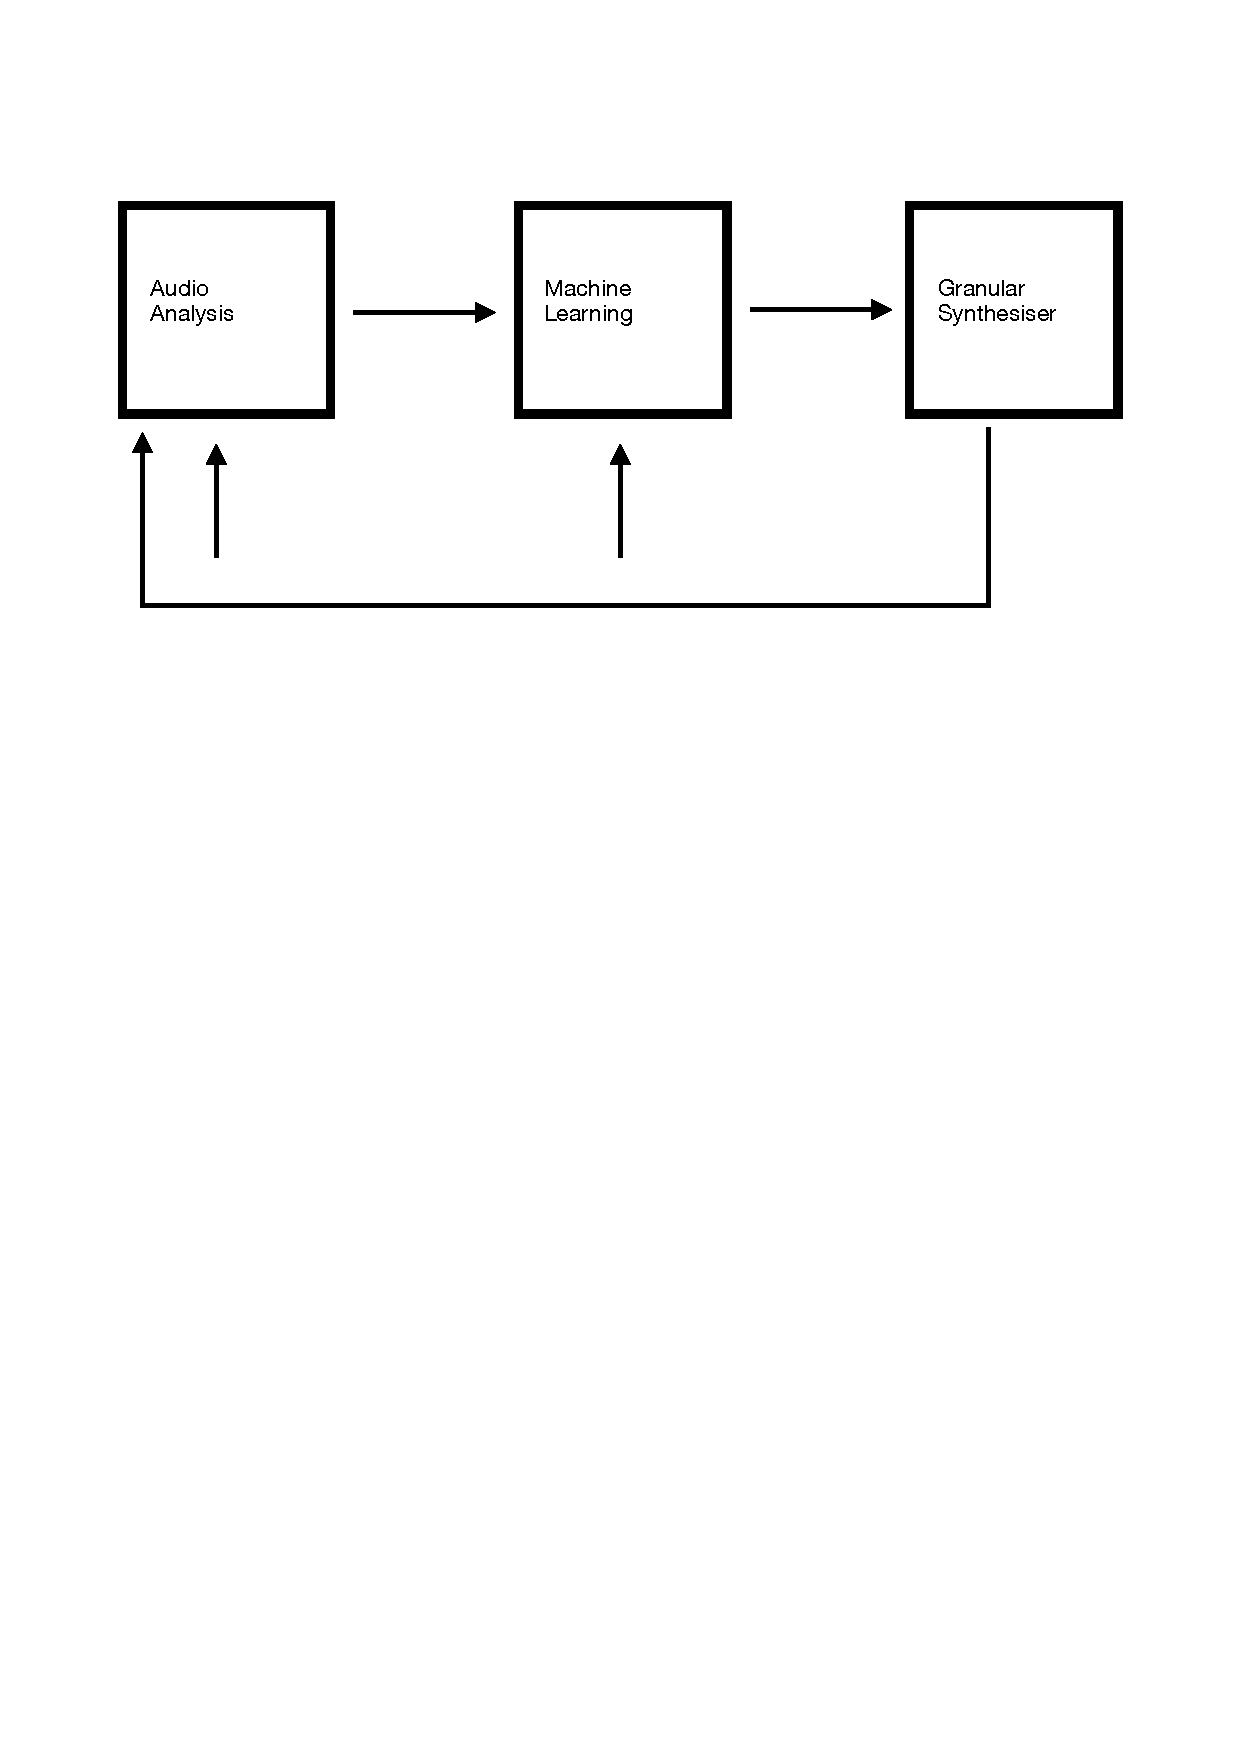
\includegraphics[width=0.5\textwidth]{images/flowchart}
\end{figure}

The box `Granular Synthesiser' in figure 1. represents a granular synthesizer.
It was implemented in C++, using the `JUCE' library.

`Machine Learning' stands for the predictions module, or more
precisely the Multilayer Perceptron model built in `Keras', and later
ported to C++ with the help of the `Frugally Deep' library.

Lastly, the `Audio Analysis' square represents the aspect of the
project responsible for extracting audio features from input
sounds. This was done with the `Essentia' library, that allowed me to
perform frame cutting, windowing, extracting the spectrum and finally
MFCCs on any specified buffer.

\section{Audio Analysis}

The only algorithm used for describing audio is the Mel-frequency
Cepstrum Coefficients. As mentioned in the Literature Review section,
it is proven to be one of the most reliable desriptors available, and
can not only describe the temporal qualities, but with the right
treatment, also be indicative of the changes that happen in the input
signal. More on that later.

In order to extract MFCCs from the signal, some preprocessing has to
be done. Namely, the signal has to be split into frames, on which the
FFT algorithm is performed. Each of the frames has to include a little
from the previous and the future one, in order to give a better
representaion of the signal. This is called a hop size.

Then, for each frame, MFCC are calculated based on the extracted
FFTs. The result for one frame is a vector of 13 floating point
values, each corresponding to a different range of frequencies.

At a sampling rate of 44.1kHz, and a buffer size of 512 samples, this
corresponds to exactly 45 vectors of 13 float values for one second of sound.

\section{Predictions}

\subsection{Dataset}

In order to get any predictions, a dataset, linking the MFCC values
with the synthesis parameters had to be created. Initially, I have set
out to create a data set of every possible combination of parameter
values, and their corresponding MFCCs. However, even though there are
only 5 adjustable parameters, with a static hop size of a tenth of
each parameter, it would take more than 1000 hours to complete this
task, given that each parameter combination would be sampled for
exactly one second.

In order to evade this limitation, a different approach was
taken. Every second, each parameter was set to a random value between
their unique minimum and maximum values. Consequently, the audio
features were extracted on each of these iterations, for exactly 10000
instances, which allowed for a creation of a dataset, of 10000
different parameter values, each corresponding to 10000 2D vectors, of
size 45 x 13 each.
%\cite{yee-king_automatic_2018}.

\subsection{Feedforward neural network}

The neural network implemented for the task of predicting the
synthesizer parameters is a Multilayer Perceptron. It's a relatively
simple, feedforward network, consiting of 3 layers.  The 45x13 MFCC
vectors served as the features, and a vector of 5 different parameter
values as the values to be predicted by the network. Firstly, the 2D
vectors, were flattened, like an image would be in a convolutional network.

Trained for 2000 epochs...
accuracy of 50\%...
parameters = this and that...
pretty shit, and not working very well, put not enough time for more experimentation...

\section{Synthesis}

\subsection{Granular Synthesis (basic explenation of the granular synth concept)}

Describing granular synthesis in one paragraph is impossible
without cutting some edges, and leaving out many intricacies of the
technique. However, a summary of sorts, describing the main concepts
behind the algorithm will be attempted here. 

Granular synthesis is an algorithm...
Grain clouds...
Xenakis...
Rodes...
Some other folks...
Capable of many thing, versatile...
graphs, graphs, graphs and pictures...

\subsection{The JUCE implementation (author's implementation)}

The granular synthesis algorithm was implemented using the `JUCE'
library. It is one of the most established libraries in the
professional audio community, being used by companies such as `Cycling
74', and `Korg' amog others(cite website?). On top of all things
audio, it provides a convenient way of creating a graphical user
interface, which was an important part of this project. Thanks to
`JUCE', the implementation was kept minimal, and elegant.

explenation of implementation...
grain class...
how grains are called...
how they are altered by the dials...
show code snippets...

\subsection{Synthesizer parameters}

There are 6 adjustable parameters...
position...
** where to spawn new grains
grain size...
** how the long are the grains spawned
position offset...
** how far away from the original position should the grains be spawned
number of grains...
** how many grain should be active at one point in time
pitch...
** how higher lower the pitch of each grain should be relative to the
original sample
global gain...
...





%What belongs in the "methods" section of a scientific paper?
%
%    Information to allow the reader to assess the believability of your results.
%    Information needed by another researcher to replicate your experiment.
%    Description of your materials, procedure, theory.
%    Calculations, technique, procedure, equipment, and calibration plots. 
%    Limitations, assumptions, and range of validity.
%    Desciption of your analystical methods, including reference to any specialized statistical software. 
%
%The methods section should answering the following questions and caveats: 
%
%    Could one accurately replicate the study (for example, all of the optional and adjustable parameters on any sensors or instruments that were used to acquire the data)?
%    Could another researcher accurately find and reoccupy the sampling stations or track lines?
%    Is there enough information provided about any instruments used so that a functionally equivalent instrument could be used to repeat the experiment?
%    If the data are in the public domain, could another researcher lay his or her hands on the identical data set?
%    Could one replicate any laboratory analyses that were used? 
%    Could one replicate any statistical analyses?
%    Could another researcher approximately replicate the key algorithms of any computer software?
%
%Citations in this section should be limited to data sources and references of where to find more complete descriptions of procedures.
%Do not include descriptions of results. 